Программы, написанные на современных языках программирования, во время выполнения могут формировать выражения на других языках и выполнять их. Языки, которые используются для написания таких динамически формируемых выражений, называются встроенными. 

Несмотря на то что сегодня широко распространено использование таких технологий, как ORM (object-relational mapping), есть области, в которых встроенные языки встречаются достаточно часто. В качестве примера можно привести реинжиниринг программного обеспечения. 

Ниже приведен пример использования встроенных языков.

\begin{figure}[h]
\label{PHP}
\centering
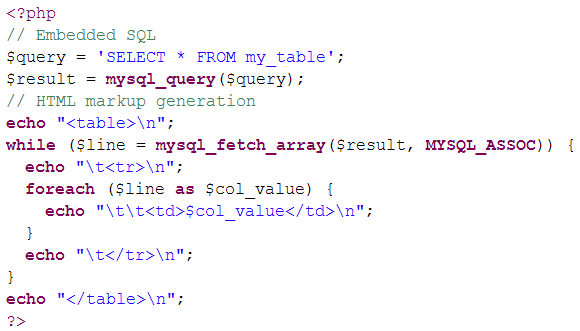
\includegraphics{Pictures/PHP.png}
\caption{Использование нескольких различных встроенных в PHP языков (MySQL, HTML)}
\end{figure}

При работе с приложениями, содержащими встроенные языки, необходимо помнить, что порождаемые строки тоже могут являться кодом на некотором языке программирования. Поэтому важно сохранить синтаксическую корректность динамически формируемых выражений. 

Одна из основных трудностей в работе со встроенными языками заключается в том, что часто отсутствуют средства разработки, позволяющие определить правильность составленного динамического выражения статическим образом, то есть до запуска основной программы. Это связано с тем, что компилятором такие выражения воспринимаются как простые строки.

С другой стороны, сегодня при создании ПО активно используются интегрированные среды разработки - IDE (Integrated Development Environment), которые предоставляют набор различной функциональности, позволяющей значительно упростить процесс создания программ. Примером могут служить такие функции, как автодополнение, рефакторинг (улучшение написанного ранее кода, не влияющее на его внешнее поведение), дополнительные статические проверки, подсказки. 

Такие возможности современных IDE были бы полезны и для встроенных языков, поскольку это позволило бы сократить время на создание, отладку и сопровождение приложений, использующих динамически формируемые выражения.  К примеру, подсветка синтаксиса могла бы сигнализировать о правильно набранной синтаксической конструкции или же о допущенной опечатке. 

В данной работе представлено механизм поддержки произвольных встроенных языков, описанных грамматикой, для среды разработки Microsoft Visual Studio \cite{MSVisualStudio}, а также описание реализации этого механизма. 
